\textbf{See the instruction for questions \inteval{\value{question}+1} to \inteval{\value{question}+2}.}

\begin{figure}[H]
    \centering
    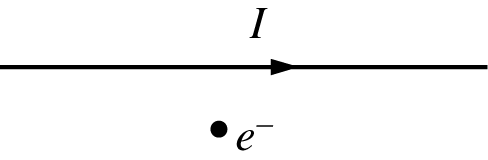
\includegraphics[scale=0.3]{images/img-009-016.png}
\end{figure}

An electron is placed near a wire carrying current $I$, as shown in the figure above, and released from rest. Both the electron and the wire are in the plane of the page.

% Multiple Choice Question 18
\begin{questions}\setcounter{question}{17}\question
Which of the following is true about the direction of the magnetic field produced by the current at the position of the electron?

\begin{choices}
\choice It is toward the top of the page.
\choice It is toward the bottom of the page.
\choice It is out of the page.
\choice It is into the page.
\choice It has no direction since there is no magnetic field at that point.
\end{choices}\end{questions}

% Multiple Choice Question 19
\begin{questions}\setcounter{question}{18}\question
Which of the following is true about the direction of the initial magnetic force acting on the electron due to the current in the wire?

\begin{choices}
\choice It is toward the top of the page.
\choice It is toward the bottom of the page.
\choice It is out of the page.
\choice It is into the page.
\choice It has no direction because the magnitude of the initial magnetic force on the electron is zero.
\end{choices}\end{questions}

